\documentclass[twocolumn]{article}
\usepackage[utf8]{inputenc}
\usepackage{amsfonts}
\usepackage{amssymb}
\usepackage{graphicx}
\usepackage{hyperref}
\usepackage{amsmath}
\usepackage{pgfplots}
\pgfplotsset{compat=1.18}
\usepackage[backend=biber, style=numeric]{biblatex}
\addbibresource{references.bib}
\usepackage{titlesec}
\titleformat{\subsection}[hang]{\normalfont\bfseries}{\thesubsection}{1em}{}
\usepackage{abstract}

\begin{document}

\title{Bunni v2: Shapeshifting AMM}
\author{zefram.eth\thanks{Thanks to Austin Adams, Sam Bacha, and 0xmons for valuable feedback.}\\ \href{mailto:zefram@baconlabs.dev}{\texttt{zefram@baconlabs.dev}}}
\date{May 2024}

\twocolumn[
    \maketitle
    \begin{onecolabstract}
Bunni v2 is a revolutionary Automated Market Maker (AMM) that introduces several groundbreaking features to optimize liquidity provision and maximize profits for liquidity providers (LPs). Building upon the concept of ticks from Uniswap v3, Bunni v2 introduces Liquidity Density Functions (LDFs) that enable efficient liquidity distribution, modification, and swaps with constant gas costs. LDFs allow LPs to provide liquidity in complex shapes and seamlessly shift or switch between these shapes, either manually or programmatically. Bunni v2 also introduces the first implementation of autonomous rebalancing, eliminating the need for external keepers, and surge fee, a solution to sandwiching during autonomous liquidity modifications. Additionally, Bunni v2 recaptures MEV and optimizes swap fee revenue using the am-AMM mechanism, uses rehypothecation for extra yield, and adopts a simple volatility-based dynamic fee model. Bunni v2 marks a new generation of ``shapeshifting" AMMs with concentrated liquidity that is automated, highly customizable, and infinitely programmable.
    \end{onecolabstract}
    \vspace{1cm}
]
\saythanks

\section{Introduction}

In 2021, Uniswap Labs deployed Uniswap v3 \cite{Adams21}, which was the first Automated Market Maker (AMM) where liquidity providers (LPs) could customize how liquidity is concentrated at different prices.

Specifically, it divides the price space into discrete ``ticks" where the price of $token_0$ in terms of $token_1$ equals $1.0001^{tick}$. Swaps within each tick is computed using the corresponding segment of a virtual constant product ($xy=k$) curve, and liquidity in a tick is defined as $\sqrt k$ of the virtual curve. Uniswap v3 LPs can create positions where liquidity is provided evenly between two ticks, which is equivalent to a larger segment of the $xy=k$ curve. Each Uniswap v3 pool can contain any number of LP positions, so the curve used by the pool when processing swaps is the aggregate of all of the $xy=k$ curve segments, effectively crowdsourced from all the LPs.

Uniswap v3 was a breakthrough in AMM development. It defined a new language for describing AMM curves and enabled LPs to provide liquidity based on their beliefs about future prices and risk appetite. It let the AMM curve of each pool be adjusted over time to strike a balance between optimizing price impact, risk, and fee revenue, as well as respond to market changes.

However, Uniswap v3 also had many shortcomings.

\begin{itemize}
  \item LP positions were restricted to provide liquidity evenly between two ticks, so providing liquidity in more complex shapes required creating \& managing multiple positions.
  \item LP positions could not be moved from one tick to another, so responding to market changes required removing the existing position, swapping tokens so the correct ratio is achieved, and creating a new position. 
  \item The gas cost, which is the fee paid for executing a transaction on the blockchain, of swaps grew linearly w.r.t. the number of ticks crossed, so larger swaps cost considerably more.
\end{itemize}

In a sense, Uniswap v3 was not quite ``automated": LPs had to frequently update their positions in order to respond to market changes. Many Automated Liquidity Managers (ALMs) such as Arrakis and Gamma were developed as a response. ALMs used automated strategies to perform the position updates in place of the human LPs. ALMs made the experience of providing liquidity better, but did not and could not address the above shortcomings.

Bunni v2 is a next generation AMM that addresses these shortcomings. \textbf{The key observation behind Bunni v2 is this: if you know exactly how liquidity is distributed across all the ticks in a pool, then it is possible to simplify a pool's aggregate curve into a single curve parametrized by a few variables.} For example, you can simplify a pool where liquidity is distributed evenly into the $xy=k$ curve. This observation enables Bunni v2 LPs to provide liquidity in complex shapes with constant gas cost. Furthermore, the ability to parametrize a pool's liquidity distribution makes it possible to shift liquidity and/or change the liquidity shape with constant gas cost, since you only need to update the values of a few parameters. The gas cost of swaps also becomes constant, since there is no longer the need to cross ticks iteratively. 

In short, Bunni v2 is the first \textit{shapeshifting AMM} where:

\begin{itemize}
  \item Liquidity can be efficiently provided in complex shapes
  \item Liquidity can be efficiently shifted regardless of the liquidity's shape, either manually or automatically using criteria like TWAP or Chainlink price oracles 
  \item Liquidity can switch from one complex shape to another, either manually or automatically
  \item The gas cost of swaps is constant
\end{itemize}

Bunni v2 introduces three breakthroughs in AMM development.

First, it introduces Liquidity Density Functions (LDFs), functions that not only define how liquidity is distributed across ticks but also make it possible to efficiently compute liquidity modifications and swaps. LDFs provide a new language for specifying liquidity distributions that builds directly on top of Uniswap v3's concept of ticks. 

Second, it introduces the first ever implementation of autonomous rebalancing, where tokens in a pool are rebalanced without requiring an external keeper to automate the execution or provide optimal swap routing. Autonomous rebalancing strips the concept of ALMs down to its essence: performing a swap when the ratio between tokens becomes extreme.

Third, it introduces surge fee as a solution to autonomous liquidity modifications being sandwiched. Surge fee makes it feasible to deploy completely onchain liquidity strategies.

Bunni v2 includes many other features, though they're not original contributions. Bunni v2 recaptures MEV and optimizes swap fee revenue using the am-AMM model introduced by Adams et al. \cite{adams2024amamm}. It implements rehypothecation where idle liquidity is deposited into external vaults to earn extra yield. It includes a simple volatility-based dynamic fee model that is used when an am-AMM manager is not present, as well as a built-in Time Weighted Average Price (TWAP) oracles.

In addition, Bunni v2 will be built on top of Uniswap v4 \cite{Adams23}, a new version of Uniswap that will enable other decentralized exchanges (DEXes) to build on top of their smart contract infrastructure. Uniswap v4 will unite DEXes around a central hub, defragmenting both orderflow and liquidity, and Bunni v2 will be a major part of this future.

The end goal of Bunni v2 is maximizing profits for LPs while minimizing complexity in the user experience. Bunni v2 is the first concentrated liquidity AMM that's both \textit{truly automated} – LPs no longer need to manually adjust positions to respond to market changes – and \textit{fully customizable} – LPs can precisely define their desired liquidity distribution and its autonomous behavior using the familiar language of ticks.

In this paper, I will go over each of the concepts mentioned above, providing details on what they are and how they work.

\section{Mathematical concepts}

\subsection{Rounded ticks (``ricks")}

In addition to dividing the price space into ticks similar to Uniswap v3, Bunni v2 is also using \textit{rounded ticks}, or ``ricks" for short. Each rick consists of $tickSpacing$ consecutive ticks and is identified by its lowest tick. Given tick $t$ and tick spacing $w$, the rick $r$ it belongs to is:
\begin{equation}
  r = \lfloor \frac{t}{w} \rfloor \cdot w  
\end{equation}
Ricks are the liquidity units used by LDFs to define liquidity distributions. By adjusting the tick spacing, pool deployers can specify the granularity to use for their liquidity distributions.

$r_{min}$ and $r_{max}$ are the minimum and maximum ricks in the rick space $R$. Given ticks $t_{min}$ and $t_{max}$ and tick spacing $w$, you can compute them like this:
\begin{equation}
  r_{min} = \lfloor \frac{t_{min}}{w} \rfloor \cdot w
\end{equation}

\begin{equation}
  r_{max} = (\lfloor \frac{t_{max}}{w} \rfloor - 1) \cdot w
\end{equation}

The reason $r_{max}$ has the $-1$ term is that ricks are defined by their lowest tick, so we need to ensure that both $r_{max}$ and $r_{max} + w$ are less than or equal to $t_{max}$.  

\subsection{Liquidity density function (LDF)}

\textit{Liquidity density functions}, or LDFs for short, are normalized functions that define how liquidity is distributed over ricks. Given a pool with tick spacing $w$ and total liquidity
\begin{equation}
  L = \sum_{r}l_r    
\end{equation}

where $l_r$ is the liquidity (as defined by Uniswap v3) at rick $r$, $l_r$ can be computed via $LDF_w: R \to [0, 1]$ in the following manner:
\begin{equation} 
  l_r = L \cdot LDF_w(r)
\end{equation}

LDFs are normalized in the sense that $\sum_r LDF_w(r) = 1$.

Another way of representing LDFs is via \textit{rick indices}. Given tick spacing $w$, rick $r$, and \textit{origin} $\mu$ (which is also a rick), its rick index $x$ is
\begin{equation}
  x = \frac{r - \mu}{w}  
\end{equation}

and an LDF can be alternatively represented as  
\begin{equation}
  d(x) = LDF_w (wx + \mu)
\end{equation}
\begin{equation}
  LDF_w (r) = d(\frac{r - \mu}{w})
\end{equation}

Rick indices make it easier to define LDFs without having to include the tick spacing as a parameter.

\subsubsection{Example: geometric distribution}

A basic LDF is the geometric distribution. Given \textit{exponent} $\alpha \in \mathbb R_{>0} \backslash \{1\}$ and \textit{length} $l \in \mathbb Z_{>0}$, the geometric LDF is defined as  
\begin{equation}
  d_{\alpha, l}(x) =
  \begin{cases}
    \frac{\alpha^x}{\frac{1 - \alpha^l}{1 - \alpha}} & x \in [0, l) \cap \mathbb Z \\
    0 & \text{otherwise}
  \end{cases}
\end{equation}

\begin{figure}
  \centering
  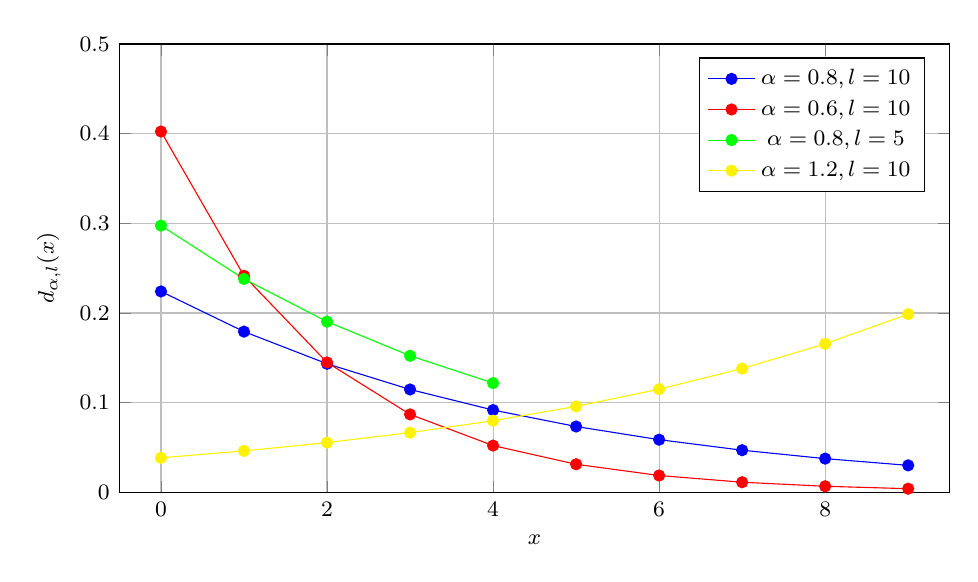
\begin{tikzpicture}
    \begin{axis}[
      xlabel={$x$},
      ylabel={$d_{\alpha, l}(x)$},
      xmin=-0.5, xmax=9.5,
      ymin=0, ymax=0.5,
      xtick={0,2,4,6,8,10},
      ytick={0,0.1,0.2,0.3,0.4,0.5},
      legend pos=north east,
      grid=major,
      width=\columnwidth,
      height=0.6\columnwidth,
      tick label style={font=\footnotesize},
      label style={font=\footnotesize},
      legend style={font=\footnotesize},
    ]
    
    \addplot[domain=0:9, samples=10, color=blue, mark=*]{0.8^x / ((1 - 0.8^10) / (1 - 0.8))};
    \addlegendentry{$\alpha = 0.8, l = 10$}
    
    \addplot[domain=0:9, samples=10, color=red, mark=*]{0.6^x / ((1 - 0.6^10) / (1 - 0.6))};
    \addlegendentry{$\alpha = 0.6, l = 10$}
    
    \addplot[domain=0:4, samples=5, color=green, mark=*]{0.8^x / ((1 - 0.8^5) / (1 - 0.8))};
    \addlegendentry{$\alpha = 0.8, l = 5$}

    \addplot[domain=0:9, samples=10, color=yellow, mark=*]{1.2^x / ((1 - 1.2^10) / (1 - 1.2))};
    \addlegendentry{$\alpha = 1.2, l = 10$}

    \end{axis}
  \end{tikzpicture}
  \caption{Geometric LDF with various parameter choices}
  \label{fig:geometric_ldf}
\end{figure}

\begin{figure}
  \centering
  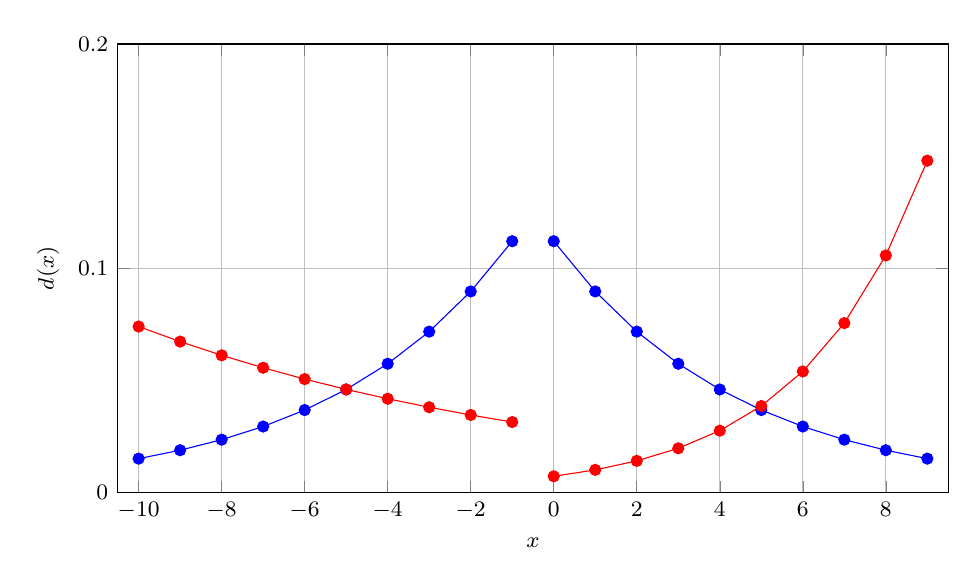
\begin{tikzpicture}
    \begin{axis}[
      xlabel={$x$},
      ylabel={$d(x)$},
      xmin=-10.5, xmax=9.5,
      ymin=0, ymax=0.2,
      xtick={-10,-8,-6,-4,-2,0,2,4,6,8,10},
      ytick={0,0.1,0.2},
      grid=major,
      width=\columnwidth,
      height=0.6\columnwidth,
      tick label style={font=\footnotesize},
      label style={font=\footnotesize},
      legend style={font=\footnotesize},
    ]
    
    \addplot[domain=-10:-1, samples=10, color=blue, mark=*]{0.5 * 0.8^(-(x+1)) / ((1 - 0.8^10) / (1 - 0.8))};
    \addplot[domain=0:9, samples=10, color=blue, mark=*]{0.5 * 0.8^x) / ((1 - 0.8^10) / (1 - 0.8))};

    \addplot[domain=-10:-1, samples=10, color=red, mark=*]{0.5 * 1.1^(-(x+1)) / ((1 - 1.1^10) / (1 - 1.1))};
    \addplot[domain=0:9, samples=10, color=red, mark=*]{0.5 * 1.4^x / ((1 - 1.4^10) / (1 - 1.4))};
    
    \end{axis}
  \end{tikzpicture}
  \caption{Double geometric LDFs, symmetric concentrated and asymmetric bid-ask}
  \label{fig:double_geometric_ldf}
\end{figure}

Essentially, the geometric LDF distributes liquidity over $l$ ricks following a geometric distribution. By adjusting the origin $\mu$, the LDF can be shifted over the rick space. By adjusting the parameters $\alpha$ and $l$, the LDF can change its shape.

For reasons that will be discussed in the following sections, the geometric LDF is particularly useful as a building block for more complex LDFs. For example, if you juxtapose two geometric LDFs and normalize them appropriately, you get a double geometric LDF that can be used to describe either a concentrated distribution or a bid-ask distribution around the origin.

This demonstrates a key feature of LDFs: they can be easily composed to create more complex distributions. In a later section I will discuss exactly how to do this.

\subsection{Cumulative amount function (CAF)}

Each LDF has two associated \textit{cumulative amount functions} (CAFs) $A_0: R \cup {r_{max}+w} \to \mathbb R_{>0}$ and $A_1: R \cup {r_{min} - w} \to \mathbb R_{>0}$, one for each token in a pool. Following Uniswap's notation, the two tokens are denoted as $token_0$ and $token_1$, and the price of $token_0$ in terms of $token_1$ equals $1.0001^{tick}$. We can compute the amount of both tokens in rick $r$ with liquidity $l_r$ in the following way:

\begin{align}
a_0(r) &= l_r \frac{\sqrt{1.0001^{r+w}} - \sqrt{1.0001^r}}{\sqrt{1.0001^{r+w}}\sqrt{1.0001^r}} \\
       &= l_r (1-1.0001^{-\frac{w}{2}})1.0001^{-\frac{r}{2}} \\
a_1(r) &= l_r (\sqrt{1.0001^{r+w}} - \sqrt{1.0001^r}) \\
       &= l_r(1.0001^\frac{w}{2} - 1) 1.0001^\frac{r}{2}
\end{align}

The cumulative amount functions at rick $\rho$ are defined as the following:

\begin{align}
A_0(\rho) &= \sum_{r = \rho}^{r_{max}} a_0(r) \\
A_1(\rho) &= \sum_{r = r_{min}}^{\rho} a_1(r)  
\end{align}

We can then expand them into:

\begin{align}
A_0(\rho) &= \sum_{r = \rho}^{r_{max}} a_0(r) \\ 
          &= \sum_{r = \rho}^{r_{max}} l_r (1-1.0001^{-\frac{w}{2}})1.0001^{-\frac{r}{2}} \\ 
          &= (1-1.0001^{-\frac{w}{2}}) L \sum_{r = \rho}^{r_{max}} LDF_w(r) 1.0001^{-\frac{r}{2}}
\end{align}
\begin{align}
A_1(\rho) &= \sum_{r = r_{min}}^{\rho} a_1(r) \\
          &= \sum_{r = r_{min}}^{\rho} l_r(1.0001^\frac{w}{2} - 1) 1.0001^\frac{r}{2} \\ 
          &= (1.0001^\frac{w}{2} - 1) L \sum_{r = r_{min}}^{\rho} LDF_w(r) 1.0001^\frac{r}{2}
\end{align}

Note that $A_0(r_{max} + w) = A_1(r_{min}-w)=0$. This is the reason the domains were extended from $R$. Also note that we can compute $\frac{A_0(\rho)}{L}$ and $\frac{A_1(\rho)}{L}$ , which are the token amounts \textit{per total liquidity unit}, without knowing $L$. We will denote them as $\frac{A_0}{L}(\rho)$ and $\frac{A_1}{L}(\rho)$.

In this form, it's easy to see why it's easy to compute $A_0$ and $A_1$ efficiently for the geometric LDF: if $d(\cdot)$ was a geometric function in $r$, we'd still have a geometric function after multiplying it by either $1.0001^{-\frac{r}{2}}$ or $1.0001^{\frac{r}{2}}$, and the sum of a geometric series has a closed form solution. It's also possible to compute them for a linear LDF, since the sum of an arithmetico-geometric sequence also has a closed form solution.

Cumulative amount functions are essential to computing liquidity modifications and swaps.

\subsection{Inverse cumulative amount function (ICAF)}

Each LDF also has two associated \textit{inverse cumulative amount functions} (ICAFs) $A_0^{-1}(\cdot)$ and $A_1^{-1}(\cdot)$. As the name suggests, they are related to the inverse functions of CAFs $A_0(\cdot)$ and $A_1(\cdot)$. However, simply using the inverse functions of CAFs is not enough for our purposes, since they only accept specific cumulative amounts that have corresponding rick indices as input, whereas we need to map all possible cumulative amounts to rick indices somehow.  The inverse functions also might not exist if the CAFs are not strictly monotonic. Thus, we define the ICAFs in the following way:

\begin{align}
A_0^{-1}(y) &= \mathrm{argmax}_{r \in R \cup \{r_{max} + w\}} \{A_0(r) : A_0(r) \geq y\} \\
A_1^{-1}(y) &= \mathrm{argmin}_{r \in R \cup \{r_{min} - w\}} \{A_1(r) : A_1(r) \geq y\}
\end{align}

How to actually compute the ICAFs depends heavily on the LDF. For geometric LDFs, the ICAFs can be computed via basic arithmetic operations in constant time. For linear LDFs, the ICAFs can be computed via arithmetic operations plus the Lambert $W$ function.

ICAFs are essential to computing swaps in constant time. Without ICAFs it's still possible to build an AMM like Bunni v2, but swaps would be much more expensive both theoretically (linear time instead of constant time) and practically (requires modifying individual Uniswap v4 positions for each rick crossed). 

\subsection{Composing distributions}

Given any two LDFs $LDF^a$ and $LDF^b$, it is possible to compose them to get a new LDF $LDF'$. Simply computing a weighted sum is enough to compute the new LDF and the corresponding CAFs:  
\begin{equation}
  LDF'(x) = w \cdot LDF^a(x) + (1-w) \cdot LDF^b(x), w \in [0, 1]
\end{equation}
\begin{equation}
  A_0'(r) = w \cdot A_0^a(r) + (1-w) \cdot  A_0^b(r), w \in [0, 1]
\end{equation}
\begin{equation}
  A_1'(r) = w \cdot A_1^a(r) + (1-w) \cdot  A_1^b(r), w \in [0, 1]
\end{equation}

Computing the new ICAFs, on the other hand, is more complicated. If we make the additional assumption that $\forall r < r_0, LDF^a(r)=0$ and $\forall r \ge r_0, LDF^b(r)=0$, then we can compute the ICAFs in the following way:
\begin{equation}
  A'^{-1}_0(y) =
    \begin{cases}
      {A_0^a}^{-1}(y) & {A_0^a}^{-1}(y) \ge r_0\\
      {A_0^b}^{-1}(y - {A_0^a}^{-1}(r_0)) & \text{otherwise} 
    \end{cases}       
\end{equation}

\begin{equation}
  A'^{-1}_1(y) =
    \begin{cases}
      {A_1^b}^{-1}(y) & {A_1^b}^{-1}(y) < r_0 \\
      {A_1^a}^{-1}(y - {A_1^b}^{-1}(r_0 - w)) & \text{otherwise}
    \end{cases}       
\end{equation}

Essentially, we're limiting the domains of the two LDFs and iterating through each LDF's ICAF to see which one produces a result that lies in its LDF's domain and is thus valid.

By repeating this binary composition process any number of LDFs can be composed together, though due to the way the ICAFs are computed the cost of computing the composite LDF's ICAFs grows linearly as we compose more LDFs into it.

\section{Liquidity modification}

Adding initial liquidity to a pool requires using the LDF to determine the correct ratio between the two tokens. After initialization, adding or withdrawing liquidity simply means adding or withdrawing some proportion of the pool's existing token reserves, which is trivial and won't be described here. 

Given input token amounts $a_0$ and $a_1$, the tick spacing $w$, the current square root price $p$, and the current tick $t$, we want to compute the maximum total liquidity $L$ we can add using these tokens. This can be done in the following process:

\begin{enumerate}
  \item Compute the rick $r$ of the current tick $t$   
    \begin{itemize}
      \item $r = \lfloor \frac{t}{w} \rfloor \cdot w$  
    \end{itemize}
  \item Compute the token densities outside rick $r$
    \begin{itemize} 
      \item $t_0=\frac{A_0}{L}(r+w), t_1=\frac{A_1}{L}(r-w)$
    \end{itemize}
  \item Compute the square root prices at ricks $r$ and $r+w$ 
    \begin{itemize}
      \item $p_r = 1.0001^{\frac r2}, p_{r+w}=1.0001^{\frac{r+w}{2}}$
    \end{itemize}   
  \item Compute the liquidity density at rick $r$
    \begin{itemize}
      \item $d_r=LDF_w(r)$
    \end{itemize}
  \item Use Uniswap math to compute the token densities inside rick $r$
    \begin{itemize}
      \item $t_0'= \frac{1}{p}-\frac{1}{p_{r+w}}, t_1'=p - p_r$  
    \end{itemize}
  \item Use the total token densities to compute $L$
    \begin{itemize}
      \item $L = \min(\frac{a_0}{t_0 + t_0'}, \frac{a_1}{t_1 + t_1'})$
    \end{itemize}
\end{enumerate}

Essentially, we compute the total token densities, i.e. how many tokens are contained in one unit of total liquidity, then divide $a_0$ and $a_1$ by the total token densities to compute their corresponding total liquidity values, and finally take the smaller of the two as the maximum total liquidity that $a_0$ and $a_1$ can support. 

In addition, the above process can be used to compute the current total liquidity of a pool given its token balances. The fact that the process works regardless of the ratio between $a_0$ and $a_1$ means that a pool's total liquidity is defined regardless of the said ratio, so the actual token ratio is independent of the ratio specified by the LDF. This property gives Bunni v2 flexibility in modifying a pool's token balances, which enables features such as shapeshifting, autonomous rebalancing, and rehypothecation.

\section{Shapeshifting} 

Shapeshifting refers to changing the liquidity distribution of a Bunni v2 pool, either manually or programmatically. Shapeshifting can take several forms:

\begin{itemize}
  \item \textbf{Shifting}: Changing the origin $\mu$ of the LDF shifts liquidity across the rick space
  \item \textbf{Morphing}: Changing the parameters of the LDF, for instance $\alpha$ and $l$ for the geometric LDF, would change the shape of the liquidity 
  \item \textbf{Switching}: Switching from one LDF to a completely different LDF
\end{itemize}

\textbf{Shapeshifting makes AMM liquidity programmable.} Developers and LPs can now design liquidity strategies suited to their specific risk profiles and beliefs, as well as automatically respond to market changes. For example, LPs can let their liquidity automatically shift to concentrate around the market price to maximize swap fee revenue, morph to decrease concentration when volatility is high and increase it when volatility is low, and/or switch between bearish LDFs and bullish LDFs to reflect changing beliefs in the market direction.

Bunni v2 is the first DEX to enable shapeshifting, and shapeshifting is the key innovation that makes Bunni v2 next-gen compared to Uniswap v3-esque AMMs.

\subsection{Interaction with other features}

When a Bunni v2 pool shapeshifts, the ratio between the two tokens in the pool will likely be different from what the updated LDF specifies, so autonomous balancing is essential for such pools. Shapeshifting also potentially exposes MEV to sandwich attackers, and surge fees \& am-AMM are used to mitigate such losses.

\section{Swaps}

At a high level, swaps are done by modifying the specified token's reserves, applying the ICAF to the updated reserves to compute the resulting rick, querying the LDF at the resulting rick to compute the resulting reserves, and calculating the difference between the current and resulting reserves to compute the actual input \& output amounts. The exact process will be described below.

Given the exact input/output flag $exactIn$ and the swap direction flag $zeroForOne$, the \textit{specified token} is $token_0$ if $exactIn = zeroForOne$ and $token_1$ otherwise. For example, given an exact input swap from $token_0$ to $token_1$, $token_0$ is the specified token since we're given an exact input amount denomoniated in $token_0$. We will look at the case when the specified token is $token_0$ and when it's $token_1$. In both cases, we will assume without loss of generality that the tokens are properly balanced according to the LDF. 

The swap has two parts: first, we use the ICAF to process swaps through an integer number of ricks; second, we use Uniswap's math to process swapping the remainder of the specified amount within the end rick.

\subsection{Specified token is $token_0$} 

Suppose the pool's current $token_0$ balance is $B_0$ and the specified amount is $b_0$. After the swap, the balance will become $B_0' = B_0 \pm b_0$, with $+$ used when $token_0$ is the input token and $-$ used when it's the output token.

\begin{enumerate}
  \item Apply the ICAF to $B_0'$ to obtain rick $r$, which is the tick the remainder of the swap will start from
    \begin{itemize}
      \item $r = A_0^{-1}(B_0')$
    \end{itemize}
  \item Use the CAF to compute the cumulative $token_0$ amount in the tick (not rick) range $[r, r_{max} + w)$  
    \begin{itemize}
      \item $A = A_0(r)$
    \end{itemize}  
  \item Use the LDF to compute the liquidity of the rick that will process the remainder of the swap
    \begin{itemize}
      \item $l = LDF_w(r - w) \cdot L$
    \end{itemize}
  \item Use Uniswap math to process swapping $B_0' - A$ from tick $r$ towards the left, i.e. $zeroForOne = true$, and obtain the resulting square root price $p$
    \begin{itemize} 
      \item $p = \frac{l}{l + (B_0' - A)\cdot p_r} p_r$
    \end{itemize}
  \item Compute the rick $r'$ which $p$ belongs to
    \begin{itemize}
      \item $t' = \log_{1.0001} p^2$
      \item $r' = \lfloor \frac{t'}{w} \rfloor \cdot w$
    \end{itemize}
  \item Compute the total token densities when the square root price is $p$
    \begin{itemize}
      \item $t_0=\frac{A_0}{L}(r'+w) + (\frac{1}{p}-\frac{1}{p_{r'+w}})$
      \item $t_1=\frac{A_1}{L}(r'-w) + (p - p_{r'})$
    \end{itemize}
  \item Compute the resulting token balances $B_0^*, B_1^*$
    \begin{itemize} 
      \item $B_0^* = Lt_0, B_1^* = Lt_1$
    \end{itemize}
  \item Compute the actual input and output amounts $b_0^*, b_1^*$
    \begin{itemize}
      \item Exact input swap: $b_0^* = B_0^* - B_0, b_1^* = B_1 - B_1^*$
      \item Exact output swap: $b_0^* = B_0 - B_0^*, b_1^* = B_1^* - B_1$  
    \end{itemize}
\end{enumerate}

\subsection{Specified token is $token_1$}

Suppose the pool's current $token_1$ balance is $B_1$ and the specified amount is $b_1$. After the swap, the balance will become $B_1' = B_1 \pm b_1$, with $+$ used when $token_1$ is the input token and $-$ used when it's the output token.

\begin{enumerate}
  \item Apply the ICAF to $B_1'$ to obtain rick $r$, which is the tick the remainder of the swap will start from
    \begin{itemize}
      \item $r = A_1^{-1}(B_1')$  
    \end{itemize}
  \item Use the CAF to compute the cumulative $token_1$ amount in the tick (not rick) range $[r_{min}, r)$
    \begin{itemize} 
      \item $A = A_1(r - w)$
    \end{itemize}
  \item Use the LDF to compute the liquidity of the rick that will process the remainder of the swap 
    \begin{itemize}
      \item $l = LDF_w(r) \cdot L$  
    \end{itemize}
  \item Use Uniswap math to process swapping $B_1' - A$ from tick $r$ towards the right, i.e. $zeroForOne = false$, and obtain the resulting square root price $p$
    \begin{itemize}
      \item $p = p_r + \frac{B_1' - A}{l}$
    \end{itemize} 
  \item Compute the rick $r'$ which $p$ belongs to
    \begin{itemize} 
      \item $t' = \log_{1.0001} p^2$
      \item $r' = \lfloor \frac{t'}{w} \rfloor \cdot w$
    \end{itemize}
  \item Compute the total token densities when the square root price is $p$
    \begin{itemize}
      \item $t_0=\frac{A_0}{L}(r'+w) + (\frac{1}{p}-\frac{1}{p_{r'+w}})$
      \item $t_1=\frac{A_1}{L}(r'-w) + (p - p_{r'})$
    \end{itemize}  
  \item Compute the resulting token balances $B_0^*, B_1^*$
    \begin{itemize}
      \item $B_0^* = Lt_0, B_1^* = Lt_1$  
    \end{itemize}
  \item Compute the actual input and output amounts $b_0^*, b_1^*$ 
    \begin{itemize}
      \item Exact input swap: $b_0^* = B_0 - B_0^*, b_1^* = B_1^* - B_1$
      \item Exact output swap: $b_0^* = B_0^* - B_0, b_1^* = B_1 - B_1^*$
    \end{itemize}
\end{enumerate}

\section{Autonomous rebalancing}

When the LDF of a pool shifts or changes shape, the current ratio between the two tokens in the pool will likely be different from what the updated LDF specifies, so rebalancing is necessary to maximize the utilization rate of the token reserves. Bunni v2 introduces \textbf{autonomous rebalancing}, which is an implementation of rebalancing that doesn't require external keepers to automate rebalances or compute the optimal swap route. Autonomous rebalancing uses Bunni v2's builtin TWAP oracle to determine when a rebalance should be initiated, and uses flood.bid, an intent-based DEX aggregator, to execute the rebalances.

\subsection{Conditions for rebalancing}

After a swap has been executed, if we detected that the LDF was updated since the previous swap, then we will compute the \textit{excess liquidity} and initiate a rebalance if it is greater than a threshold proportion of the total liquidity.

The excess liquidity of a pool is defined as the minimum total liquidity that can be supported by the excess tokens. Note that due to how total liquidity is computed, there is at most one token in a pool that can be in excess. Given excess $token_0$ amount $a_0$, the excess liquidity $e_0$ can be computed in the following way:
\begin{equation}
  e_0 = \min_r \frac{a_0}{\frac{A_0}{L}(r)} = \frac{a_0}{\max_r \frac{A_0}{L}(r)} = \frac{a_0}{\frac{A_0}{L}(r_{min})}
\end{equation}

Likewise, given excess $token_1$ amount $a_1$, the excess liquidity $e_1$ can be computed in the following way: 
\begin{equation}
  e_1 = \min_r \frac{a_1}{\frac{A_1}{L}(r)} = \frac{a_1}{\max_r \frac{A_1}{L}(r)} = \frac{a_1}{\frac{A_1}{L}(r_{max})}  
\end{equation}

Rebalance is initiated if $\max(\frac{e_0}{L}, \frac{e_1}{L}) \ge \tau$, where $\tau$ is some threshold value.

\subsection{Rebalance parameters}

Given some amount of the excess token, we want to swap some portion of it into the other token in the pool such that the resulting tokens match the ratio specified by the LDF. This is computed via the following process (without loss of generality we will assume $token_0$ is the excess token):

\begin{enumerate}
  \item Query the TWAP oracle to get the average square root price $\bar p$ and the corresponding rick $\bar r$
  \item Compute total token densities using the TWAP value
    \begin{itemize}
      \item $t_0=\frac{A_0}{L}(\bar r+w) + (\frac{1}{\bar p}-\frac{1}{p_{\bar r+w}})$
      \item $t_1=\frac{A_1}{L}(\bar r-w) + (\bar p - p_{\bar r})$  
    \end{itemize}
  \item Compute target token amounts $g_0$ and $g_1$
    \begin{itemize}
      \item $g_0 = e_0t_0, g_1=e_0t_1$
    \end{itemize}
  \item Submit intent to swap $a_0-g_0$ of $token_0$ for at least $\gamma g_1$ of $token_1$
    \begin{itemize} 
      \item $\gamma \in (0, 1]$ is the slippage parameter
    \end{itemize}
\end{enumerate}

The TWAP value is used in evaluating the LDF instead of the spot price in order to prevent manipulation.

\subsection{Swap execution}

Executing optimal swaps initiated from a smart contract is a difficult problem. When liquidity for a token is spread across multiple exchanges and token pairs, obtaining the optimal swap route requires both a lot of information and a lot of computation, neither of which a smart contract can easily access. Bunni v2 uses flood.bid, an intent-based DEX aggregator, to execute swaps during rebalancing. Intent-based solutions such as flood.bid allow Bunni v2 to broadcast a swap intent onchain and let offchain solvers provide optimal swap execution.  

However, currently flood.bid does not provide a way for a smart contract to verify that the swap provided by the solver is indeed optimal, so a malicious solver could execute the rebalance swap with the worst possible slippage. Bunni v2 addresses this by only allowing a whitelisted set of solvers execute rebalance swaps. This whitelist is mostly set by governance, but the am-AMM manager of a pool is also automatically part of the whitelist for that pool. This makes rebalance swaps partially permissionless, since the am-AMM manager of a pool is selected via a permissionless auction. It also ensures that any MEV from rebalance swaps can be recaptured via am-AMM auctions.

\section{Surge fee}

When the liquidity of a pool is autonomously updated in any way (i.e. when a ``surge" occurs), be it from LDF updates, rehypothecation yields, or autonomous rebalances, a sandwiching opportunity may occur where an attacker can sandwich the update with two swaps and make a profit. In order to address this issue, Bunni v2 introduces \textbf{surge fee}. Bunni v2 essentially starts a dutch auction every time a pool surges, where the swap fee is increased to a large value and decreases over time back to normal. Any profitable sandwich attack will likely be executed immediately after the swap fee equals the attack profit, allowing LPs to recover the vast majority of the losses.

Given the current timestamp $t$, the timestamp of the most recent surge $t_{surge}$, the timestamp of the most recent swap $t_{swap}$, the surge autostart time $\tau_{auto}$, the max surge fee $f_{sMax}$, and the surge half-life $\tau$, the surge fee is:
\begin{equation}
  f_{surge} = f_{sMax} \exp_2(-\frac{t - \min(t_{surge}, t_{swap} + \tau_{auto})}{\tau})  
\end{equation}

where $\exp_2$ is the exponential function with base 2.

To compute the swap fee with surge fee applied, simply take the max of the surge fee and the regular swap fee $f_0$:
\begin{equation}
  f = \max(f_{surge}, f_0) 
\end{equation}

Essentially, when a surge occurs the swap fee is increased to $f_{sMax}$ and then decreases exponentially with a half-life of $\tau$ until the normal fee level is reached.  

The $\min(t_{surge}, t_{swap} + \tau_{auto})$ term requires explanation. Because a surge can occur at any time (e.g. due to the TWAP oracle updating over time) but Bunni v2 only gets to execute code when a swap occurs, we don't have access to the true $t_{surge}$ value and can only estimate it by using the timestamp of the first swap after a surge occurs. This means that if we simply used $t_{surge}$ to compute $f_{surge}$, the first swap after a surge will always be charged a surge fee of $f_{sMax}$, effectively halting swaps completely unless someone is willing to make a tiny swap and pay the high swap fee + gas fee. Using $\min(t_{surge}, t_{swap} + \tau_{auto})$ instead means if the first swap after a surge is executed more than $\tau_{auto}$ seconds since the most recent swap, we assume that the surge occured at timestamp $t_{swap} + \tau_{auto}$. In this way, the surge fee automatically begins exponentially decreasing after $t_{swap} + \tau_{auto}$, which avoids halting swaps for more than $\tau_{auto}$ seconds plus however long it takes for the swap fee to catch a bid.

\section{Rehypothecation}

Bunni v2 uses ERC-4626\cite{ERC4626} vaults to implement \textbf{rehypothecation}, which means depositing idle assets into external vaults to earn additional yield. Yield-generating protocols such as Aave\cite{Aave}, Yearn\cite{Yearn}, and Gearbox\cite{Gearbox} can be used for rehypothecation. Rehypothecation is particularly easy for Bunni v2 to implement versus other concentrated liquidity AMMs such as Uniswap v3, due to its flexibility with its token reserves as mentioned in the liquidity modification section.

\subsection{Rebalancing between vault reserves and raw tokens}

When rehypothecation is enabled for a token, some portion of the pool's reserves is stored in the vault specified by the pool creator, while the rest is stored as raw tokens to facilitate swaps. After each swap, the pool rebalances tokens between the vault reserves and the raw tokens. For each token in a pool with rehypothecation enabled, there are three parameters that define its rebalance behavior: $\phi_{min}, \phi_{max}, \phi_{target}$. When the ratio
\begin{equation}
\phi = \frac{rawTokenBalance}{totalBalance}  
\end{equation}

goes outside of the range $[\phi_{min}, \phi_{max}]$, the token is rebalanced between the vault reserves and the raw tokens so that $\phi = \phi_{target}$. This is a simple but effective strategy for rebalancing that ensures some level of raw tokens in the pool such that reasonably sized swaps can be processed without expensive vault operations.

\subsection{Advantages}

One question some may ask is why rehypothecation is needed, since you can achieve a similar effect by creating regular AMM pools that use yield bearing tokens (e.g. wrapped Aave aETH)? There are three reasons why rehypothecation provides a superior solution:

\begin{enumerate}
  \item Pools sharing the same underlying asset (e.g. ETH) but using different protocols to earn extra yield (e.g. Aave, Gearbox) can still route swaps through each other via the common asset.
  \item As vaults earn yield, there is no need to adjust pool pricing to reflect the yield accrual, since the price is denominated in the underlying assets instead of the vault share tokens.
  \item Swappers more often want to swap from/to raw assets (e.g. ETH) instead of vault share tokens, so rehypothecation makes swaps cheaper overall by maintaining a balance of raw tokens.
\end{enumerate}

\subsection{Interaction with other features}

Bunni v2 pools that use rehypothecation for one or both tokens should enable autonomous rebalancing to maximize token utilization, unless the yield rate of both tokens is similar. Pools using rehypothecation for both tokens also need to enable surge fees, since total liquidity will increase over time as yield accrues.

\section{am-AMM}

The Auction-Managed Automated Market Maker (am-AMM) by Adams et al. \cite{adams2024amamm} is ``a single mechanism that targets two important unsolved problems for AMMs: reducing losses to informed orderflow, and maximizing revenue from uninformed orderflow". Bunni v2 pools implement the am-AMM mechanism. This paper will not go into detail how am-AMM works, but will give a high-level overview.

\subsection{MEV recapture}

am-AMM enables Bunni v2 to recapture MEV by giving the manager—decided via competitive auction–a privileged position in capturing the MEV, be it from arbitrages or from rebalancing swaps. Because the manager is decided via competitive auction, LPs will indirectly receive the MEV via the auction proceeds.

\subsection{Swap fee optimization}

The am-AMM manager of a pool receives all of its swap fee revenue and has the ability to set the swap fee value. Bunni v2 also allows the manager to set \textbf{directional} swap fees, such that swapping from $token_0$ to $token_1$ may have a different swap fee than swapping from $token_1$ to $token_0$. The am-AMM manager is incentivized to maximize the swap fee revenue, since the manager would receive all of it. This offloads swap fee optimization to offchain actors. The LPs benefit from the increased swap fee revenue since they receive it indirectly via the auction proceeds.  

\subsection{Surge fees}

The surge fees mechanism is meant to protect LPs from sandwiching attacks when surges occur, but if an am-AMM manager is present then the MEV losses from surges can be recovered via the auction proceeds. In Bunni v2, the am-AMM manager of a pool may enable or disable surge fees.

\subsection{Withdrawal fee}

In order to prevent LPs from strategically withdrawing liquidity when arbitrage opportunities occur and hurt the income of the am-AMM manager, there needs to be a withdrawal fee. Adams et al. \cite{adams2024amamm} were able to derive the minimum required withdrawal fee for a constant-product AMM, but applying the same process to Bunni v2 does not yield a result due to the large space of liquidity distributions supported. Therefore, Bunni v2 implements a withdrawal delay instead as Adams et al. have suggested, which enables managers to monitor withdrawal transactions and execute arbitrages while the withdrawal is still in queue. This delay only needs to be on the order of a few blocks, since that's more than enough time to execute an arbitrage.

\section{Volatility-based swap fee}

\begin{figure}
  \centering
  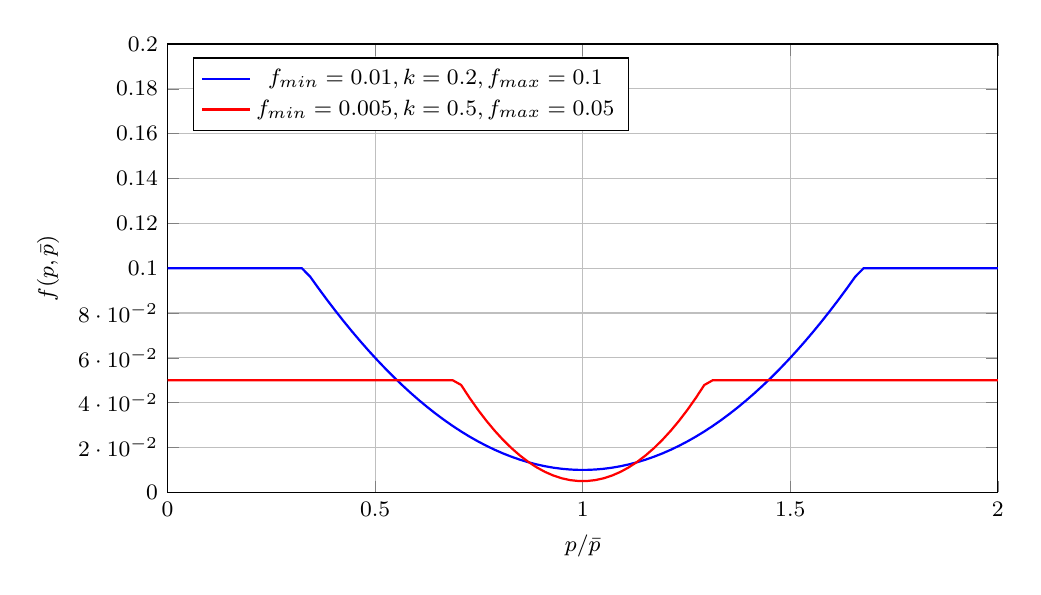
\begin{tikzpicture}
    \begin{axis}[
      xlabel={$p / \bar{p}$},
      ylabel={$f(p, \bar{p})$},
      xmin=0, xmax=2,
      ymin=0, ymax=0.2,
      xtick={0,0.5,1,1.5,2},
      ytick={0,0.02,0.04,0.06,0.08,0.1,0.12,0.14,0.16,0.18,0.2},
      legend pos=north west,
      grid=major,
      width=\columnwidth,
      height=0.6\columnwidth,
      tick label style={font=\footnotesize},
      label style={font=\footnotesize},
      legend style={font=\footnotesize},
      domain=0:2,
      samples=100,
    ]
    
    \addplot[color=blue, thick] {min(0.01 + 0.2 * (x - 1)^2, 0.1)};
    \addlegendentry{$f_{min} = 0.01, k = 0.2, f_{max} = 0.1$}
    
    \addplot[color=red, thick] {min(0.005 + 0.5 * (x - 1)^2, 0.05)};
    \addlegendentry{$f_{min} = 0.005, k = 0.5, f_{max} = 0.05$}
    
    \end{axis}
  \end{tikzpicture}
  \caption{Volatility-based swap fee with various parameter shoices}
  \label{fig:dynamic_fee_model}
\end{figure}

Bunni v2 includes a volatility-based dynamic swap fee mechanism that is used in the absence of an am-AMM manager. It increases the swap fee quadratically as the pool's spot price deviates from the TWAP value. The swap fee can be calculated via the following formula:
\begin{equation}
  f(p, \bar p) = \min (f_{min} + k \cdot (\frac{p}{\bar p} - 1)^2, f_{max})
\end{equation}

where $f(\cdot)$ returns the fee percentage charged from a swap, $p$ is the spot price of the pool after the swap, $\bar p$ is the TWAP of the pool, and $f_{min}, k, f_{max}$ are parameters that are non-negative, with $f_{min} \le f_{max}$.

Essentially, this is a quadratic fee model that's bounded in the range $[f_{min}, f_{max}]$. It charges higher fees for swaps that push the spot price away from the TWAP and lower fees for swaps that push the spot price towards the TWAP. It is particularly responsive to volatility, since if a large swap away from the TWAP immediately gets charged a higher swap fee.

This is by no means a perfect model for a volatility-based swap fee, but it provides a reasonable default that makes use of Bunni v2's built-in TWAP oracle. Introducing a volatility oracle and using that for computing the swap fee may provide a better result, but it would be inferior to what an am-AMM manager can do using an offchain model that can be arbitrarily complex.

\section{Example scenarios}

Given the numerous features available to Bunni v2 LPs it may be difficult for a beginner to design liquidity positions for a given scenario.  Below are a few example scenarios and liquidity positions that are appropriate for them.

\subsection{Low-risk stable pair: USDT/USDC}

USDT (Tether)\cite{Tether} and USDC (Circle)\cite{Circle} are two well-established stablecoins whose prices are pegged to the US dollar. While they both have had depeg events in the past where their prices went significantly below 1 USD, they have been by far the most stable and liquid stablecoins.

\begin{figure}
  \centering
  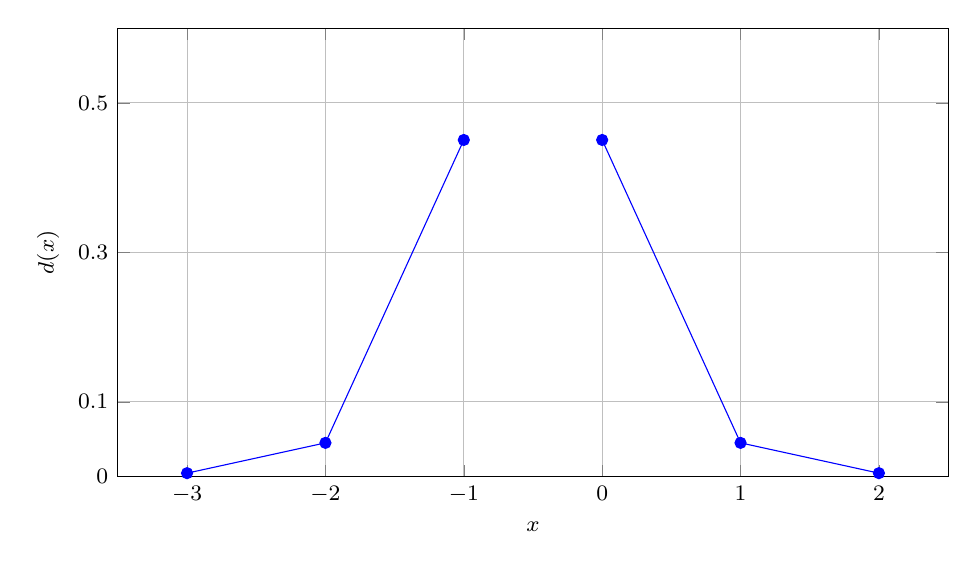
\begin{tikzpicture}
    \begin{axis}[
      xlabel={$x$},
      ylabel={$d(x)$},
      xmin=-3.5, xmax=2.5,
      ymin=0, ymax=0.6,
      xtick={-3,-2,-1,0,1,2},
      ytick={0,0.1,0.3,0.5},
      grid=major,
      width=\columnwidth,
      height=0.6\columnwidth,
      tick label style={font=\footnotesize},
      label style={font=\footnotesize},
      legend style={font=\footnotesize},
    ]
    
    \addplot[domain=-3:-1, samples=3, color=blue, mark=*]{0.5 * 0.1^(-(x+1)) / ((1 - 0.1^3) / (1 - 0.1))};
    \addplot[domain=0:2, samples=3, color=blue, mark=*]{0.5 * 0.1^x) / ((1 - 0.1^3) / (1 - 0.1))};

    \end{axis}
  \end{tikzpicture}
  \caption{LDF for a low-risk stable pair (e.g. USDT/USDC)}
  \label{fig:low_risk_stable}
\end{figure}

\subsubsection{Liquidity distribution}

The best liquidity position for a USDT/USDC pair would be a static double-geometric distribution that's heavily concentrated around the price of 1 USDT/USDC or even a flat distribution. This way, the position is optimized for providing the best quotes and attracting swap volume, with no regard for impermanent loss since there won't be any for such a low-risk stable pair.

Because the liquidity distribution is static, there is no need to enable autonomous rebalancing.

\subsubsection{Rehypothecation}

Low-risk stable pairs often attract lots of liquidity since there is evergreen demand for earning yield on USD with low risk, which means the yield will likely be massively diluted, so it makes sense to use rehypothication to earn extra yield. Lending platforms like Aave offer yield on USDC and USDT with low risk.

An example parameter choice for rehypothecation is $\phi_{min}=5\%, \phi_{target}=10\%, \phi_{max}=15\%$. If the pool has \$100m of liquidity and the raw token ratio is at $\phi_{target}$, then \$90m would be earning yield on Aave and \$10m would be sitting in the pool waiting to be swapped with, and the pool would be able to handle swaps up to \$5m in either direction without triggering a vault rebalance.

\subsection{High-risk stable pair: eETH/ETH}

eETH (Etherfi ETH)\cite{Etherfi} is a token pegged to 1 ETH (Ether) issued by Etherfi, a liquidity restaking protocol that earns yield via ETH restaking. Users can earn yield on eETH by depositing it into a vault that returns weETH (wrapped eETH) which increases in value over time. Users can also instantly mint eETH using ETH at a 1:1 exchange rate, meaning the price of eETH can never significantly exceed 1 ETH. Compared to USDT/USDC the risk of eETH depegging from ETH is higher due to Etherfi being a newer protocol.

\begin{figure}
  \centering
  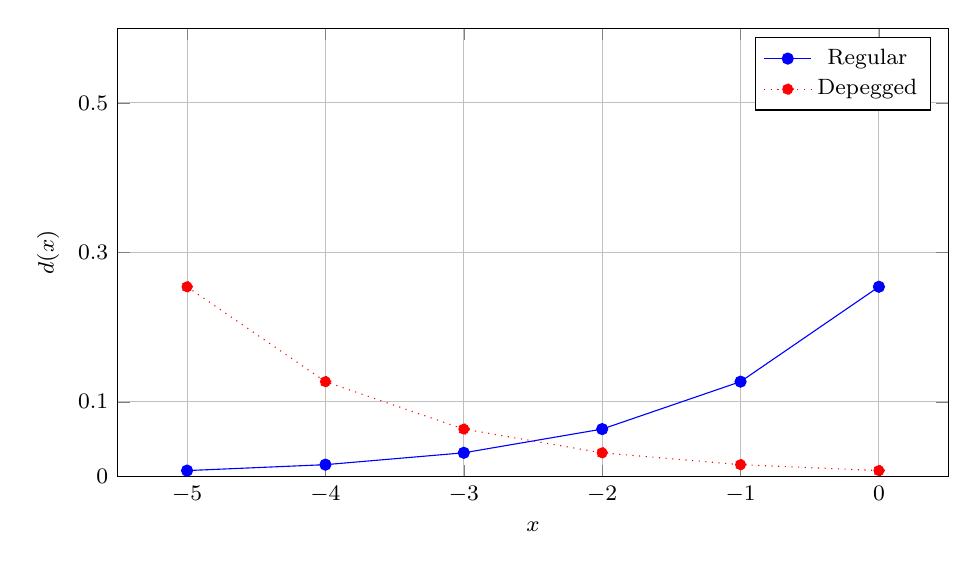
\begin{tikzpicture}
    \begin{axis}[
      xlabel={$x$},
      ylabel={$d(x)$},
      xmin=-5.5, xmax=0.5,
      ymin=0, ymax=0.6,
      xtick={-5,-4,-3,-2,-1,0},
      ytick={0,0.1,0.3,0.5},
      grid=major,
      width=\columnwidth,
      height=0.6\columnwidth,
      tick label style={font=\footnotesize},
      label style={font=\footnotesize},
      legend style={font=\footnotesize},
    ]
    
    \addplot[domain=-5:0, samples=6, color=blue, mark=*]{0.5 * 0.5^(-x)) / ((1 - 0.5^6) / (1 - 0.5))};
    \addlegendentry{Regular}
    \addplot[domain=-5:0, samples=6, color=red, mark=*, dotted]{0.5 * 0.5^(x+5)) / ((1 - 0.5^6) / (1 - 0.5))};
    \addlegendentry{Depegged}

    \end{axis}
  \end{tikzpicture}
  \caption{LDF for a high-risk stable pair (e.g. eETH/ETH) or yield pair (e.g. rETH/ETH) with "buy-the-dip" behavior}
  \label{fig:high_risk_stable}
\end{figure}

\subsubsection{Liquidity distribution}

There's no need to provide significant liquidity for when 1 eETH $>$ 1 ETH, due to the availability of minting eETH. Thus, it's best to use a geometric distribution where the maximum liquidity density occurs around price 1 ETH/eETH and gradually decreases as the price of eETH decreases. Using this distribution there would be no liquidity for prices $>$ 1 ETH/eETH. Alternatively, a double geometric distribution can be used to allocate a small portion of the liquidity to the $>$ 1 ETH/eETH region to facilitate a smoother swapping experience. Liquidity is more efficiently utilized by not wasting any of it on LPing at unlikely prices.

Because eETH is expected to be pegged at 1 ETH, there is no need to enable shifting or switching. However, it may be advisable to enable morphing to protect LPs against the risk of depegging. The pool can detect when a depeg occurs to eETH by comparing the TWAP value to the peg; if a depeg did occur, the pool can update the $\alpha$ value of the geometric LDF such that liquidity is concentrated at some price below 1 ETH/eETH, which enables the pool to allocate more funds towards bidding eETH at a lower price. In other words, the pool can automatically "buy the dip" if eETH depegs. If eETH regains peg after depegging, the pool can automatically return to the regular distribution. This "buy the dip" behavior protects LPs from depegs and potentially even enables LPs to profit from them, and if a depeg never happens then the pool would behave the same as a static pool. Thus it always makes sense to enable it. Do note that the lower the liquidity density at the peg, the more effective the protection, so there exists a tradeoff between risk and reward.

The TWAP window size for morphing should be set to a small value, such as 1-5 minutes, because depeg events can occur very rapidly.

Autonomous rebalancing doesn't need to be enabled, since the only time when the pool's tokens can go out of balance is when a depeg event occurs, which will likely be infrequent and temporary.

\subsubsection{Rehypothecation}

It makes sense to enable rehypothecation for eETH via the weETH vault, which lets LPs earn yield from Eigenlayer. It's also possible to enable it for ETH via lending protocols like Aave and Gearbox.

Because the majority of swaps is expected to be from eETH to ETH, LPs should set a higher $\phi_{target}$ for ETH and a lower $\phi_{target}$ for eETH to facilitate low gas cost swaps.

\subsection{Yield pair: rETH/ETH}

rETH (Rocket Pool staked ETH)\cite{RocketPool} is a liquid staking token that accrues yield from ETH staking. Unlike eETH, which is always pegged to 1 ETH, rETH's price increases over time to reflect yield accrual. For example, if the ROI since the creation of rETH is 10\% then the price of rETH would be 1.1 ETH.

\subsubsection{Liquidity distribution}

We can use an asymmetric distribution similar to the eETH/ETH pool to reflect our assumption that the price of rETH will not significantly exceed the peg. However, the price that rETH is pegged to increases over time as yield is accrued, so shifting should be enabled to regularly reconcentrate liquidity at the latest peg. Fetching the latest peg value is straightforward since the rETH smart contract exposes a \texttt{getExchangeRate()} function that returns the up-to-date peg value. Autonomous rebalancing should be also enabled, since shifting will make the pool's tokens go out of balance.

The "buy-the-dip" behavior can also be enabled to protect against depeg events.

\subsubsection{Rehypothecation}

There is likely no need to rehypothecate rETH since it already accrues yield from ETH staking. ETH can be rehypothecated via lending platforms like Aave and Gearbox. Like the eETH/ETH pool, the rETH/ETH pool should use a higher $\phi_{target}$ for ETH to facilitate low gas cost swaps.

\subsection{Major volatile pair: ETH/USDC}

ETH (Ether)\cite{EthereumWhitepaper} is a major cryptocurrency with a market cap of several hundred billion dollars and regularly sees tens of billions of dollars in daily trading volume (as of May 2024). Its price is determined by market forces and is in no way pegged to any other asset, therefore it is volatile in dollar terms.

\begin{figure}
  \centering
  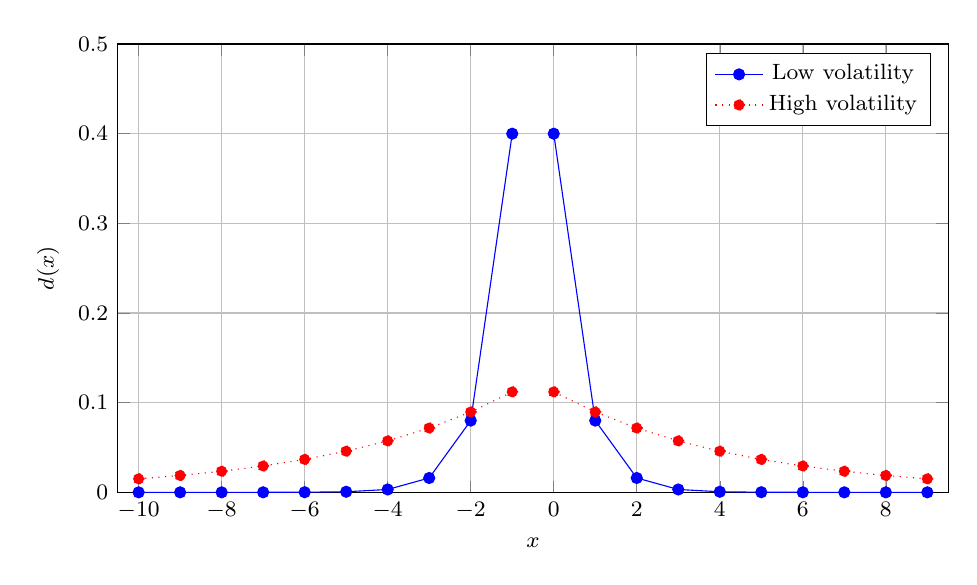
\begin{tikzpicture}
    \begin{axis}[
      xlabel={$x$},
      ylabel={$d(x)$},
      xmin=-10.5, xmax=9.5,
      ymin=0, ymax=0.5,
      xtick={-10,-8,-6,-4,-2,0,2,4,6,8,10},
      ytick={0,0.1,0.2,0.3,0.4,0.5},
      grid=major,
      width=\columnwidth,
      height=0.6\columnwidth,
      tick label style={font=\footnotesize},
      label style={font=\footnotesize},
      legend style={font=\footnotesize},
    ]
    
    \addplot[domain=-10:-1, samples=10, color=blue, mark=*]{0.5 * 0.2^(-(x+1)) / ((1 - 0.2^10) / (1 - 0.2))};
    \addlegendentry{Low volatility}

    \addplot[domain=-10:-1, samples=10, color=red, mark=*, dotted]{0.5 * 0.8^(-(x+1)) / ((1 - 0.8^10) / (1 - 0.8))};
    \addlegendentry{High volatility}

    \addplot[domain=0:9, samples=10, color=blue, mark=*]{0.5 * 0.2^x) / ((1 - 0.2^10) / (1 - 0.2))};

    \addplot[domain=0:9, samples=10, color=red, mark=*, dotted]{0.5 * 0.8^x) / ((1 - 0.8^10) / (1 - 0.8))};
    
    \end{axis}
  \end{tikzpicture}
  \caption{LDF for a major volatile pair (e.g. ETH/USDC). Liquidity concentration decreases when volatility increases.}
  \label{fig:major_volatile}
\end{figure}

\subsubsection{Liquidity distribution}

The main goal of an LP in the ETH/USDC pool is to maximize the swap fee revenue while managing the risks from impermanent loss and volatility. There are many different ways to provide liquidity for volatile token pairs and there is no one-size-fit-all solution, so I will provide an example strategy that makes sense theoretically and demonstrates what is possible to execute using Bunni v2 but may not work out in practice.

We can use a symmetric double-geometric distribution that's concentrated at some price, which we can set to either the TWAP value or an oracle-provided value using oracle solutions such as Chainlink. This enables the pool to be competitive in its quotes and thus attract non-toxic swap volume, even when the price of ETH deviates from the price that the pool is currently concentrated around. The pool can also morph its liquidity based on the volatility of ETH, measured via some onchain or offchain oracle, such that the liquidity becomes less concentrated when the volatility increases. The liquidity can even change from being concentrated at the oracle price to being concentrated away from it if the price of ETH becomes too volatile, so that the potential impermanent loss is decreased. Given the dynamic liquidity distribution, autonomous rebalancing will have to be enabled.

\subsubsection{Rehypothecation}

There are many different sources of yield for ETH and USDC, usually lending platforms like Aave and Gearbox. Given that ETH is a major cryptocurrency, its volatility is lower compared to less major ones, so it should be safe to enable rehypothecation for both ETH and USDC with a moderate $\phi_{target}$ around 25-50\%.

\subsection{Minor volatile pair: GEAR/ETH}

GEAR (Gearbox)\cite{Gearbox} is the governance token of Gearbox Finance, a modular leverage protocol. Compared to ETH, GEAR is a much more minor cryptocurrency, with a market cap on the order of tens of millions of dollars (as of May 2024). Like ETH, the price of GEAR is determined by the market and is thus volatile. Unlike ETH, GEAR is directly connected with a team with vested interest in ensuring the token is liquid, and does not see so much trading volume such that deep liquidity can be counted on without intervention from the team. As a result, the Gearbox team has been incentivizing liquidity using GEAR. Autonomous rebalancing should be enabled to accomodate for the shifting behavior.

\subsubsection{Liquidity distribution}

Given that LPs receive incentives in GEAR and that the GEAR/ETH pool is created by the Gearbox team, theres is less consideration for impemanent loss and more focus on ensuring the liquidity of GEAR. Therefore, a simple double-geometric distribution concentrated around the oracle price can be used. The liquidity distribution can be asymmetric so that slightly more weight is given to the ETH side of the pool, which translates to more bids for GEAR.  

\subsubsection{Rehypothecation}

It makes sense to disable rehypothecation for GEAR. Firstly, there aren't many yield opportunities for GEAR. Secondly, disabling rehypothecation makes it cheaper gas-wise for users to buy GEAR, which the Gearbox team likely desires. Rehypothecation should be enabled for ETH to make providing liquidity for GEAR more attractive, and the $\phi_{target}$ parameter can be lower (e.g. 5\%) to both increase the rehypothecation yield and discourage selling GEAR into ETH (since the gas cost would be slightly higher).

\section{Conclusion}

The release of Bunni v2 marks a new generation of shapeshifting AMMs with concentrated liquidity that is automated, highly customizable, and infintely programmable. It is another leap forward in making onchain market making not only profitable but competitive with offchain market making, as well as simplifying the user experience of providing liquidity. Bunni v2 does all this while retaining the permissionlessness, transparency, and composability of past AMMs. It offers developers and researchers a new language for specifying the behavior of AMM liquidity, encouraging further innovations in the space.

Bunni v2 and its am-AMM also marks a paradigm shift in the field of MEV. AMMs have been the largest source of MEV by far, and it has been extracted by unaligned bots that have no incentive to give it back. am-AMM formalizes the MEV extraction process and enables LPs to recover most of the value, which will significantly decrease the overall amount of MEV. Bunni v2 fundamentally realigns MEV incentives, allowing benign arbitrage while recapturing parasitic value extraction for the benefit of LPs and the protocol.

Built on the bedrock of Uniswap v4's unified liquidity infrastructure and powered by innovations like LDFs and am-AMM, Bunni v2 aims to be more than just an incremental upgrade. It is a quantum leap ahead, synthesizing the best ideas in DeFi into an elegant and expressive protocol that will change market making forever. Bunni v2 is not just a new AMM design - it is a glimpse of an achievable future where decentralized exchanges dominate: one with deep liquidity, smart automation, fair incentives, and a seamless experience for all. The future of DeFi is shapeshifting, and it begins now with Bunni v2.

\printbibliography

\end{document}